\PassOptionsToPackage{unicode=true}{hyperref} % options for packages loaded elsewhere
\PassOptionsToPackage{hyphens}{url}
%
\documentclass[]{book}
\usepackage{lmodern}
\usepackage{amssymb,amsmath}
\usepackage{ifxetex,ifluatex}
\usepackage{fixltx2e} % provides \textsubscript
\ifnum 0\ifxetex 1\fi\ifluatex 1\fi=0 % if pdftex
  \usepackage[T1]{fontenc}
  \usepackage[utf8]{inputenc}
  \usepackage{textcomp} % provides euro and other symbols
\else % if luatex or xelatex
  \usepackage{unicode-math}
  \defaultfontfeatures{Ligatures=TeX,Scale=MatchLowercase}
\fi
% use upquote if available, for straight quotes in verbatim environments
\IfFileExists{upquote.sty}{\usepackage{upquote}}{}
% use microtype if available
\IfFileExists{microtype.sty}{%
\usepackage[]{microtype}
\UseMicrotypeSet[protrusion]{basicmath} % disable protrusion for tt fonts
}{}
\IfFileExists{parskip.sty}{%
\usepackage{parskip}
}{% else
\setlength{\parindent}{0pt}
\setlength{\parskip}{6pt plus 2pt minus 1pt}
}
\usepackage{hyperref}
\hypersetup{
            pdftitle={A To Be Determined Title of Bas's PhD Thesis},
            pdfauthor={Bas Machielsen},
            pdfborder={0 0 0},
            breaklinks=true}
\urlstyle{same}  % don't use monospace font for urls
\usepackage{color}
\usepackage{fancyvrb}
\newcommand{\VerbBar}{|}
\newcommand{\VERB}{\Verb[commandchars=\\\{\}]}
\DefineVerbatimEnvironment{Highlighting}{Verbatim}{commandchars=\\\{\}}
% Add ',fontsize=\small' for more characters per line
\usepackage{framed}
\definecolor{shadecolor}{RGB}{248,248,248}
\newenvironment{Shaded}{\begin{snugshade}}{\end{snugshade}}
\newcommand{\AlertTok}[1]{\textcolor[rgb]{0.94,0.16,0.16}{#1}}
\newcommand{\AnnotationTok}[1]{\textcolor[rgb]{0.56,0.35,0.01}{\textbf{\textit{#1}}}}
\newcommand{\AttributeTok}[1]{\textcolor[rgb]{0.77,0.63,0.00}{#1}}
\newcommand{\BaseNTok}[1]{\textcolor[rgb]{0.00,0.00,0.81}{#1}}
\newcommand{\BuiltInTok}[1]{#1}
\newcommand{\CharTok}[1]{\textcolor[rgb]{0.31,0.60,0.02}{#1}}
\newcommand{\CommentTok}[1]{\textcolor[rgb]{0.56,0.35,0.01}{\textit{#1}}}
\newcommand{\CommentVarTok}[1]{\textcolor[rgb]{0.56,0.35,0.01}{\textbf{\textit{#1}}}}
\newcommand{\ConstantTok}[1]{\textcolor[rgb]{0.00,0.00,0.00}{#1}}
\newcommand{\ControlFlowTok}[1]{\textcolor[rgb]{0.13,0.29,0.53}{\textbf{#1}}}
\newcommand{\DataTypeTok}[1]{\textcolor[rgb]{0.13,0.29,0.53}{#1}}
\newcommand{\DecValTok}[1]{\textcolor[rgb]{0.00,0.00,0.81}{#1}}
\newcommand{\DocumentationTok}[1]{\textcolor[rgb]{0.56,0.35,0.01}{\textbf{\textit{#1}}}}
\newcommand{\ErrorTok}[1]{\textcolor[rgb]{0.64,0.00,0.00}{\textbf{#1}}}
\newcommand{\ExtensionTok}[1]{#1}
\newcommand{\FloatTok}[1]{\textcolor[rgb]{0.00,0.00,0.81}{#1}}
\newcommand{\FunctionTok}[1]{\textcolor[rgb]{0.00,0.00,0.00}{#1}}
\newcommand{\ImportTok}[1]{#1}
\newcommand{\InformationTok}[1]{\textcolor[rgb]{0.56,0.35,0.01}{\textbf{\textit{#1}}}}
\newcommand{\KeywordTok}[1]{\textcolor[rgb]{0.13,0.29,0.53}{\textbf{#1}}}
\newcommand{\NormalTok}[1]{#1}
\newcommand{\OperatorTok}[1]{\textcolor[rgb]{0.81,0.36,0.00}{\textbf{#1}}}
\newcommand{\OtherTok}[1]{\textcolor[rgb]{0.56,0.35,0.01}{#1}}
\newcommand{\PreprocessorTok}[1]{\textcolor[rgb]{0.56,0.35,0.01}{\textit{#1}}}
\newcommand{\RegionMarkerTok}[1]{#1}
\newcommand{\SpecialCharTok}[1]{\textcolor[rgb]{0.00,0.00,0.00}{#1}}
\newcommand{\SpecialStringTok}[1]{\textcolor[rgb]{0.31,0.60,0.02}{#1}}
\newcommand{\StringTok}[1]{\textcolor[rgb]{0.31,0.60,0.02}{#1}}
\newcommand{\VariableTok}[1]{\textcolor[rgb]{0.00,0.00,0.00}{#1}}
\newcommand{\VerbatimStringTok}[1]{\textcolor[rgb]{0.31,0.60,0.02}{#1}}
\newcommand{\WarningTok}[1]{\textcolor[rgb]{0.56,0.35,0.01}{\textbf{\textit{#1}}}}
\usepackage{longtable,booktabs}
% Fix footnotes in tables (requires footnote package)
\IfFileExists{footnote.sty}{\usepackage{footnote}\makesavenoteenv{longtable}}{}
\usepackage{graphicx,grffile}
\makeatletter
\def\maxwidth{\ifdim\Gin@nat@width>\linewidth\linewidth\else\Gin@nat@width\fi}
\def\maxheight{\ifdim\Gin@nat@height>\textheight\textheight\else\Gin@nat@height\fi}
\makeatother
% Scale images if necessary, so that they will not overflow the page
% margins by default, and it is still possible to overwrite the defaults
% using explicit options in \includegraphics[width, height, ...]{}
\setkeys{Gin}{width=\maxwidth,height=\maxheight,keepaspectratio}
\setlength{\emergencystretch}{3em}  % prevent overfull lines
\providecommand{\tightlist}{%
  \setlength{\itemsep}{0pt}\setlength{\parskip}{0pt}}
\setcounter{secnumdepth}{5}
% Redefines (sub)paragraphs to behave more like sections
\ifx\paragraph\undefined\else
\let\oldparagraph\paragraph
\renewcommand{\paragraph}[1]{\oldparagraph{#1}\mbox{}}
\fi
\ifx\subparagraph\undefined\else
\let\oldsubparagraph\subparagraph
\renewcommand{\subparagraph}[1]{\oldsubparagraph{#1}\mbox{}}
\fi

% set default figure placement to htbp
\makeatletter
\def\fps@figure{htbp}
\makeatother

\usepackage{booktabs}
\usepackage[]{natbib}
\bibliographystyle{apalike}

\title{A To Be Determined Title of Bas's PhD Thesis}
\author{Bas Machielsen}
\date{2020-09-26}

\begin{document}
\maketitle

{
\setcounter{tocdepth}{1}
\tableofcontents
}
\hypertarget{preface}{%
\chapter{Preface}\label{preface}}

This is a to be written preface to Bas's future PhD thesis, which is also available in .pdf and .epub (add links in the future) formats by clicking the download button below. The .pdf version is an exact copy of the paper version.

I have created this page in part to facilitate the access to my work, in part to learn how to work properly with \texttt{R}'s \texttt{bookdown} package, and in part because of environmental reasons. Many people prefer to read online anyway.

I put in a lot of acknowledgements in my preface, but I also want to make a point about open access, transparency, reproducibility, and a clean workflow as vital elements to a PhD trajectory.

\hypertarget{intro}{%
\chapter{Introduction}\label{intro}}

You can label chapter and section titles using \texttt{\{\#label\}} after them, e.g., we can reference Chapter \ref{intro}. If you do not manually label them, there will be automatic labels anyway, e.g., Chapter \ref{methods}.

Figures and tables with captions will be placed in \texttt{figure} and \texttt{table} environments, respectively.

\begin{Shaded}
\begin{Highlighting}[]
\KeywordTok{par}\NormalTok{(}\DataTypeTok{mar =} \KeywordTok{c}\NormalTok{(}\DecValTok{4}\NormalTok{, }\DecValTok{4}\NormalTok{, }\FloatTok{.1}\NormalTok{, }\FloatTok{.1}\NormalTok{))}
\KeywordTok{plot}\NormalTok{(pressure, }\DataTypeTok{type =} \StringTok{'b'}\NormalTok{, }\DataTypeTok{pch =} \DecValTok{19}\NormalTok{)}
\end{Highlighting}
\end{Shaded}

\begin{figure}

{\centering 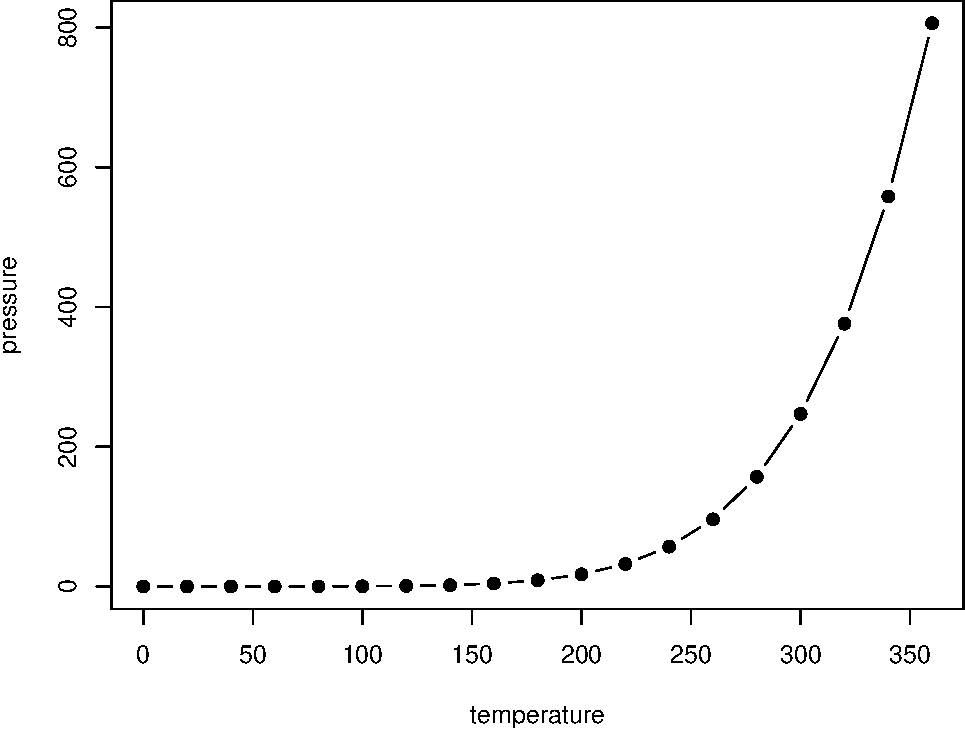
\includegraphics[width=0.8\linewidth]{phd_thesis_files/figure-latex/nice-fig-1} 

}

\caption{Here is a nice figure!}\label{fig:nice-fig}
\end{figure}

Reference a figure by its code chunk label with the \texttt{fig:} prefix, e.g., see Figure \ref{fig:nice-fig}. Similarly, you can reference tables generated from \texttt{knitr::kable()}, e.g., see Table \ref{tab:nice-tab}.

\begin{Shaded}
\begin{Highlighting}[]
\NormalTok{knitr}\OperatorTok{::}\KeywordTok{kable}\NormalTok{(}
  \KeywordTok{head}\NormalTok{(iris, }\DecValTok{20}\NormalTok{), }\DataTypeTok{caption =} \StringTok{'Here is a nice table!'}\NormalTok{,}
  \DataTypeTok{booktabs =} \OtherTok{TRUE}
\NormalTok{)}
\end{Highlighting}
\end{Shaded}

\begin{table}

\caption{\label{tab:nice-tab}Here is a nice table!}
\centering
\begin{tabular}[t]{rrrrl}
\toprule
Sepal.Length & Sepal.Width & Petal.Length & Petal.Width & Species\\
\midrule
5.1 & 3.5 & 1.4 & 0.2 & setosa\\
4.9 & 3.0 & 1.4 & 0.2 & setosa\\
4.7 & 3.2 & 1.3 & 0.2 & setosa\\
4.6 & 3.1 & 1.5 & 0.2 & setosa\\
5.0 & 3.6 & 1.4 & 0.2 & setosa\\
\addlinespace
5.4 & 3.9 & 1.7 & 0.4 & setosa\\
4.6 & 3.4 & 1.4 & 0.3 & setosa\\
5.0 & 3.4 & 1.5 & 0.2 & setosa\\
4.4 & 2.9 & 1.4 & 0.2 & setosa\\
4.9 & 3.1 & 1.5 & 0.1 & setosa\\
\addlinespace
5.4 & 3.7 & 1.5 & 0.2 & setosa\\
4.8 & 3.4 & 1.6 & 0.2 & setosa\\
4.8 & 3.0 & 1.4 & 0.1 & setosa\\
4.3 & 3.0 & 1.1 & 0.1 & setosa\\
5.8 & 4.0 & 1.2 & 0.2 & setosa\\
\addlinespace
5.7 & 4.4 & 1.5 & 0.4 & setosa\\
5.4 & 3.9 & 1.3 & 0.4 & setosa\\
5.1 & 3.5 & 1.4 & 0.3 & setosa\\
5.7 & 3.8 & 1.7 & 0.3 & setosa\\
5.1 & 3.8 & 1.5 & 0.3 & setosa\\
\bottomrule
\end{tabular}
\end{table}

You can write citations, too. For example, we are using the \textbf{bookdown} package \citep{R-bookdown} in this sample book, which was built on top of R Markdown and \textbf{knitr} \citep{xie2015}.

\hypertarget{wodpe}{%
\chapter{The Wealth of the Dutch Political Elite}\label{wodpe}}

Here comes paper 1: the Wealth of the Dutch Political Elite.

To do:

\begin{itemize}
\item
  Find how footnotes work.
\item
  Find how citations with bibtex work.
\end{itemize}

\hypertarget{the-political-elite-and-the-welfare-state}{%
\chapter{The Political Elite and the Welfare State}\label{the-political-elite-and-the-welfare-state}}

Here, paper 2: voting behavior and the political elite, it's role in the establishment of democracy and the welfare state.

\hypertarget{political-rents-under-a-changing-electoral-regime}{%
\chapter{Political Rents Under A Changing Electoral Regime}\label{political-rents-under-a-changing-electoral-regime}}

\textbf{Abstract:}
Numerous studies have shown evidence indicating that politicians profit financially from holding office by extracting rents. The mechanisms by which politicians extract these rents, however, remain unclear. In this paper, I focus on one possible determinant of political rents: electoral openness and competition. Exploiting a multitude of district-level elections in the 19th century Netherlands, and using a sample of {[}number{]} close elections, I use a regression discontinuity design to investigate the influence of being politically active on personal wealth at the end of politicians' lives relative to runners-up, that is, individuals who wanted to become politically active. I relate the results to various electoral reforms that were enacted over the course of the late 19th and early 20th centuries, which culminated in universal suffrage. I find that political rents decrease as the electoral arena opens up. I conduct several robustness analyses.

\hypertarget{introduction}{%
\section{Introduction}\label{introduction}}

In the majority of modern constitutions around the world, it is stipulated that the people of a given country have the power to decide what happens to their country. In practice, however, such direct forms of governance are hardly ever implemented, and national rule involves some delegation of power from the people to representatives, politicians, who are in turn expected to act in the interest of those who elected them. In many cases, this turns out to be only partially true. Politicians are often suspected to use and abuse their political position for private gain, or otherwise pursue policies that are counter to the interests of their constituents. Indeed, numerous studies have shown the existence of particular forms of political rents, that is to say, benefits accruing to politicians beyond their formal compensation. Although often suspected to be monetary, political rents can take on many forms, including, but not limited to advantaging certain firms and sectors, creating excess employment, ignoring certain preferences of the electorate and prioritizing one's own, engaging in discretionary spending to increase their chances at reelection, and in more extreme cases, sabotage or otherwise tilt the playing field in favor of incumbent politicians over newcomers.

Throughout modern history, accusations of politicians' abuse of power have not escaped the attention of politicians themselves either. Many attempts have been made by politicians to regulate themselves in order to minimize or altogether root out abuse of power, the most prominent and often-used being of course regular elections. Regular elections are assumed to ensure at least some degree of accountability by providing politicians with an incentive to act in such a way as to increase their chances of being reelected. Elections, however, are not a panacea. Under many circumstances, elections fail to adequately reduce abuse of power by politicians, for example, in the case of failure of relevant information about politicians' performance reaching the general public. Elections are not the only mechanisms that politicians, political theorists and economists have come up with: several other mechanisms aimed at ensuring accountability include term limits, to prevent the same individuals from holding power too long, asset disclosure laws, to force politicians to disclose information about their wealth, its origin and its evolution, the institution of a publicly accessible debate, for example in an assembly or lower house, or a free press to disseminate relevant and trustworthy information. Furthermore, constitutions itself can be thought of as a device to enact constraints on the behavior of politicians as well as the general public. Other institutions that are present in a large number of countries include a senate, or other independent judicial organs that yield various degrees of power to ensure judicial coherence of laws. In many countries, there are also various restrictions on eligibility: it is often the case that a member of parliament cannot simultaneously serve as an executive. Finally, supranational institutions can also be thought of attempts at constraining national politicians' behavior and at ensuring that the rights of certain constituencies are respected.

All of the aforementioned instruments are often thought to play an important role in reducing corruption and improving democratic accountability, but politicians have also used the very same instruments at their disposal to entrench themselves or have otherwise distorted those institutions. Some examples involve delaying, annulling or falsifying elections, or constraining the elections so as to place certain restrictions on candidates belonging to a certain gender or religion, or on a minimum amount of wealth. Propaganda can also be thought of as interference with the purpose of the press, that is, disseminating relevant and trustworthy information.

The effect of yet other mechanisms can be thought of as ambiguous: one case in point is the institution of a salary or other compensation for politicians: one the one hand, salaries are expected to increase the independence of politicians in face of attempts at bribery or other attempts at pressuring a politician. On the other hand, remuneration might attract less trustworthy or lower-ability individuals to politics that might not have the best interests of the constituents at heart, or otherwise induces shirking on the part of politicians. Another example of an institution of which the mechanisms at work are not clear are political parties: political parties and associated party discipline serve as an additional constraint on elected politicians: political party membership can be thought of as a bargain between the party and an individual politician: a party might help an individual with political aspirations get elected by providing a platform to disseminate information about the individual's ideologies, policies and ideas. In return, the politician offers the party their popularity and the promise of broadly supporting the party's entire program (regardless of their views on any specific policy). Should the politician renege on this bargain, the party can decide to oust the politician. A competing perspective on the function of political parties argues that political parties can restrict the set of available policies, or force politicians to act in the party's interest, rather than in the interest of their constituents.

In this paper, I investigate a subset of the aforementioned mechanisms: I attempt to find what the influence is of eligibility and suffrage regimes and political parties on the ability of politicians to extract rents using a specific case in history: the road towards universal suffrage in the Netherlands in the late 19th and early 20th centuries. The Netherlands started out as a country under absolute monarchy in the early 19th century, but switched to constitutional monarchy and parliamentary control following liberal reforms in 1848. This meant by no means that the country met present-day standards in terms of democratic accountability: there were severe restrictions to suffrage in the most important governmental bodies: one had to be male, and pay a minimum amount of taxes to be accorded the right to vote, although eligibility was (theoretically) completely unconstrained. In the other governmental body, however, eligibility restrictions also applied: contrary to the lower house, there were restrictions on eligibility, again related to the amount of taxes paid. Throughout the late 19th and early 20th centuries, politicians have campaigned for, and ultimately achieved, universal suffrage. This happened in several stages: electoral reforms were enacted in 1887 and 1896 before universal male suffrage was introduced in 1917 and universal suffrage in 1918. I relate these different electoral regimes to regression discontinuity estimates of political rents {[}explain before what this is{]} to find out whether average political rents decreases after opening up the political arena to more and more stringent competition.

This same period also saw the development and dissemination of political parties. As the differences between liberal and confessional (Christian) factions of parliament mounted, politicians and politically conscious citizens began to organize themselves into election associations (\textit{Kiesvereenigingen}), the existence of which was quickly superseded by political parties as we know them today: the first political party, the Anti-Revolutionary Party (ARP) was founded in 1879. The existence of political parties can have important consequences for political behavior, and by relating the RDD estimates to variation in party allegiance, I investigate what the influence of political parties are on the ability of politicians to extract rents.

The results show that

{[}{[}Results{]}{]}

The remainder of this study is structured as follows. First, in section 2, we discuss the historical background by focusing on (i) the details of eligibility and suffrage restrictions and their evolution over time, (ii) electoral associations and the origins political parties, and (iii) the logic and system of elections in the district system, which was active until 1917. In section 3, we introduce the methodology. In section 4, we show the results and investigate various alternative explanations. In section 5, we conclude.

\hypertarget{methodology}{%
\section{Methodology}\label{methodology}}

We employ three different procedures to estimate the average treatment effect of being elected into national politics on personal wealth: first, we employ a natural matching procedure and traditional regression analysis: this entails that we find close elections, and for every close elections, we find the candidate \(i\), who (i) marginally won, and the candidate \(j\), who was the runner-up, and compute the average treatment effect as:

\[ \text{ATE} = \displaystyle\sum_{e = 1}^{E} W_{iet} - W_{jet} \]

In other words, we sum over all close elections \(\{e, \dots, E\}\), which took place at time \(t\), the difference between the wealth of the elected politician \(i\) and the runner-up \(j\), and we standardize the wealth to an estimate at the time of the election to account for differences in age of death.

Second, we employ a synthetic matching procedure, which involves matching all winners to similar losers on the basis of district and demographic variables. For a large subsection of runners-up, we were able to find their profession, using various sources, their date of birth, and their date of decease. This provides us with natural covariates with the help of which we can decompose the ATE. Crucially, we further decompose the effect by electoral period, and political party of the winner. (HISCLASS)

Thirdly, we employ a regression discontinuity design (RDD):

\hypertarget{prci}{%
\chapter{Political Rents in Colonial Indonesia}\label{prci}}

\hypertarget{r-markdown}{%
\section{R Markdown}\label{r-markdown}}

This is an R Markdown document. Markdown is a simple formatting syntax for authoring HTML, PDF, and MS Word documents. For more details on using R Markdown see \url{http://rmarkdown.rstudio.com}.

When you click the \textbf{Knit} button a document will be generated that includes both content as well as the output of any embedded R code chunks within the document. You can embed an R code chunk like this:

\begin{Shaded}
\begin{Highlighting}[]
\KeywordTok{summary}\NormalTok{(cars)}
\end{Highlighting}
\end{Shaded}

\begin{verbatim}
##      speed           dist       
##  Min.   : 4.0   Min.   :  2.00  
##  1st Qu.:12.0   1st Qu.: 26.00  
##  Median :15.0   Median : 36.00  
##  Mean   :15.4   Mean   : 42.98  
##  3rd Qu.:19.0   3rd Qu.: 56.00  
##  Max.   :25.0   Max.   :120.00
\end{verbatim}

\hypertarget{including-plots}{%
\section{Including Plots}\label{including-plots}}

You can also embed plots, for example:

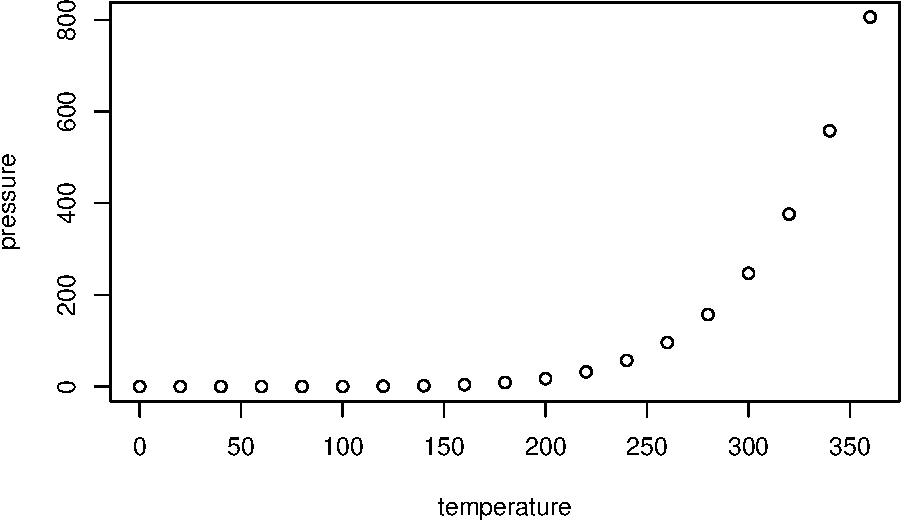
\includegraphics{phd_thesis_files/figure-latex/pressure-1.pdf}

Note that the \texttt{echo\ =\ FALSE} parameter was added to the code chunk to prevent printing of the R code that generated the plot.

\hypertarget{final-words}{%
\chapter{Final Words}\label{final-words}}

We have finished a nice book.

\hypertarget{dutchsum}{%
\chapter{Dutch Summary}\label{dutchsum}}

\hypertarget{r-markdown-1}{%
\section{R Markdown}\label{r-markdown-1}}

This is an R Markdown document. Markdown is a simple formatting syntax for authoring HTML, PDF, and MS Word documents. For more details on using R Markdown see \url{http://rmarkdown.rstudio.com}.

When you click the \textbf{Knit} button a document will be generated that includes both content as well as the output of any embedded R code chunks within the document. You can embed an R code chunk like this:

\begin{Shaded}
\begin{Highlighting}[]
\KeywordTok{summary}\NormalTok{(cars)}
\end{Highlighting}
\end{Shaded}

\begin{verbatim}
##      speed           dist       
##  Min.   : 4.0   Min.   :  2.00  
##  1st Qu.:12.0   1st Qu.: 26.00  
##  Median :15.0   Median : 36.00  
##  Mean   :15.4   Mean   : 42.98  
##  3rd Qu.:19.0   3rd Qu.: 56.00  
##  Max.   :25.0   Max.   :120.00
\end{verbatim}

\hypertarget{including-plots-1}{%
\section{Including Plots}\label{including-plots-1}}

You can also embed plots, for example:

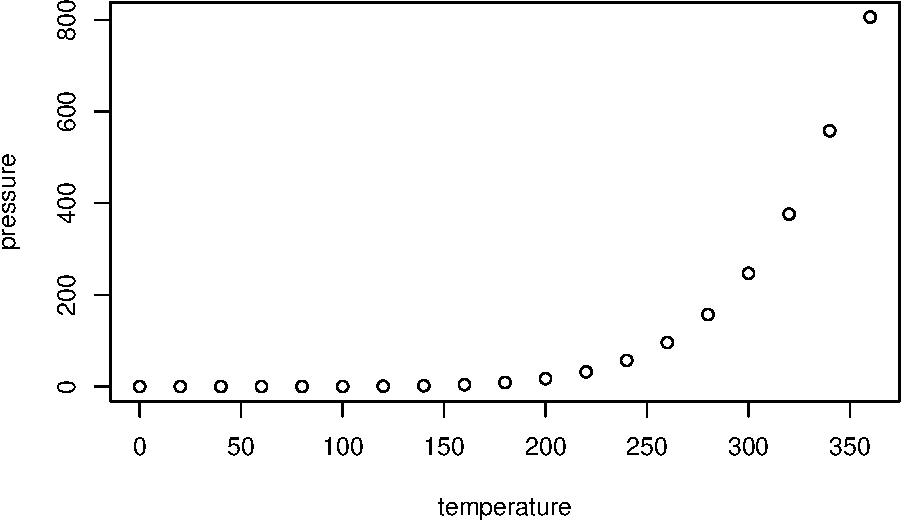
\includegraphics{phd_thesis_files/figure-latex/pressure1-1.pdf}

Note that the \texttt{echo\ =\ FALSE} parameter was added to the code chunk to prevent printing of the R code that generated the plot.

\bibliography{book.bib,packages.bib}

\end{document}
